% DUET -- Introduction (DAC 2027 draft, 2026-10-20)
% (2026-11-14) DRAM cost/power: zns (ATC'21), leaftl (ASPLOS'23 Sec. 1-2), solidigm-csal ("added DRAM will increase SSD price
% and power consumption"). Board area: E1.S / E3 specs fix the card size. micron-iu only says the 1:1000 ratio is "no longer
% sustainable" (no cost, power, or area), so it no longer backs this sentence. LMB (arXiv 2406.02039, DapuStor, preprint)
% says on-board DRAM is limited by space near the controller, cited for board area (user, 2026-11-14).
% Numbers: results/paper_dac/tables.md (NVMeVirt, 12.5% mapping DRAM, OP 7%). TODO-marked cites need sources.
% Class numbers: best FTL of each class per workload (on-demand = DFTL, LeaFTL; hybrid = FAST, CoMap; coarse IU = IU+RMW).
% Read 2.4x = min(DFTL, LeaFTL) / DUET avg read, max over workloads (YCSB-B). p99 write 4.6x = FAST / DUET on TPC-C. FAST = FAST-B12 (same budget). FAST full (cache_bytes=1e9, results/final_fastfull): 72%, 2.7x.

\section{Introduction}
\label{sec:intro}
% (2026-11-14, user) motivation paragraph for large QLC SSDs. Verified wording: meta-qlc "The growth of data and need for
% increased power efficiency are leading to innovative storage solutions."; solidigm-122tb "Data storage power, thermal and
% space constraints are accelerating as AI adoption increases.", "3.4X more terabytes per watt versus 30TB TLC", "up to 4
% petabytes of storage per one rack unit", "up to 84 percent less storage power in network-attached storage (NAS)
% deployments versus legacy hybrid HDD + TLC solutions".
% (2026-11-14, user) restructured: demand -> QLC -> however, DRAM limit -> FTL / page-level mapping -> table size.
% (2026-11-14, user) 10X AI-model sentence dropped (brief footnote [3] cites a Towards Data Science blog on parameter counts).
% solidigm-122tb: "high-capacity SSDs for AI and other data-intensive workloads", "Data storage power, thermal and space
% constraints are accelerating as AI adoption increases". solidigm-p5336-brief (2023, verified on the page): "The D5-P5336 delivers TLC-equivalent performance for read and
% data-intensive workloads", "more sustainable storage infrastructure than both TLC SSD- and HDD-based solutions".
% solidigm-122tb: "3.4X more terabytes per watt versus 30TB TLC". No verified per-watt number versus HDDs.
Data centers store a rapidly growing amount of data~\cite{idc-dataage}, and AI
workloads further raise the demand for large and fast storage~\cite{dsi,solidigm-122tb}. The power and space of data center storage,
however, are limited~\cite{dsi,meta-qlc,solidigm-122tb}. High-capacity quad-level cell (QLC) SSDs
store more data than HDDs and triple-level cell (TLC) SSDs within the same power
and space~\cite{meta-qlc,solidigm-122tb,solidigm-p5336-brief}, and provide read
performance close to that of TLC SSDs~\cite{solidigm-p5336-brief}.
A 122\,TB QLC SSD, for example, stores 3.4$\times$ more
data per watt than a 30\,TB TLC SSD and uses up to 84\% less power than hybrid HDD
storage~\cite{solidigm-122tb}. SSDs of
64 and 128\,TB are being released and developed~\cite{solidigm-122tb,samsung-bm1743}.
% (2026-11-14, user: compare with HDDs) solidigm-122tb: "Consumes up to 84 percent less storage power in network-attached
% storage (NAS) deployments versus legacy hybrid hard-disk drive (HDD) + TLC solutions". No verified per-watt or per-rack
% number versus HDD alone (P5336 brief footnotes give only drive-level power inputs).

However, high-capacity SSDs cannot hold the conventional page-level mapping table of
their flash translation layer (FTL) in on-device DRAM. The FTL maps each logical address of the host to a
physical address, because NAND flash must erase a whole block before it is
overwritten, and thus every update is written out of place.
Conventional SSDs use page-level mapping, which keeps one map entry for every 4\,KB
page in on-device DRAM. For a high-capacity SSD, this table grows too large. A 128\,TB SSD has $2^{35}$ logical pages,
so each entry needs at least 35 bits and the table takes 140\,GB. Providing this much on-device DRAM is impractical because
of its cost and power~\cite{zns,leaftl,solidigm-csal} and the fixed board area of data
center form factors~\cite{sff-e1s,sff-e3,lmb}, so high-capacity SSDs have to translate
addresses with a mapping DRAM budget that is only a fraction of the full page-level
mapping table (Figure~\ref{fig:intro}a).

\begin{figure}[t]
  \centering
  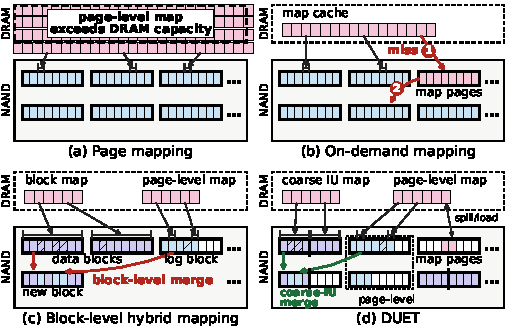
\includegraphics[width=\columnwidth]{figs/fig_intro.pdf}
  \vspace{-6mm}
  \caption{Address translation of four FTLs. In (d), page-level mappings are evicted
  to map pages instead of being merged when the DRAM table is full, and are loaded back on access.}
  \label{fig:intro}
  \vspace{-5mm}
\end{figure}

% Existing techniques reduce the mapping DRAM, but each of them pays for it in
% latency.
Existing techniques reduce the size of the mapping table in DRAM, but each of them increases either read or write latency.
\emph{On-demand mapping}~\cite{dftl,leaftl,cftl} (Figure~\ref{fig:intro}b) keeps the whole page-level mapping table in flash and caches part of it in an on-device map cache.
A read whose mapping is not in the on-device DRAM needs an extra flash read
before its data read, so its read latency spikes.
\emph{Block-level hybrid mapping}~\cite{fast,janusftl,superblock}
(Figure~\ref{fig:intro}c), on the other hand, maps most data
per NAND block and appends updates to page-mapped log blocks. When free space
runs low, the log blocks are merged back into their data blocks, and a merge
must copy all valid pages of a whole NAND block. These copies compete with host writes, so write latency grows.
The third technique is the \emph{uniform coarse indirection unit} (uniform coarse IU) of
\mbox{16--64\,KB}, which many recent commercial high-capacity SSDs
use~\cite{micron-iu,solidigm-csal,solidigm-p5336-spec}. Each map entry points to a
coarse IU instead of a page. When a write is smaller than a coarse IU, however, the
FTL reads the rest of the unit, merges the new data, and writes the whole unit again
(read-modify-write, RMW). This still increases write latency.
% (2026-11-13, reviewer: too long) Moved to Section 2: FAST p99 write 3--4x Page under random I/O. Already in Section 2:
% synchronous map-miss read, NAND block growth [pen], P5336 32 KB IU, 1/8 DRAM, RMW raises WA.

We present \textbf{DUET} (\textbf{DU}al-granularity \textbf{E}conomical
\textbf{T}ranslation), an FTL that keeps two mapping granularities, the coarse IU
and the 4\,KB page, under a fixed mapping DRAM budget (Figure~\ref{fig:intro}d). DUET maps most data
per coarse IU and writes small writes out of place as 4\,KB pages, so the host write
path has no RMW. All coarse-IU mappings and most page-level mappings stay in
on-device DRAM, so DUET needs far fewer mapping reads than on-demand mapping.
DUET merges 4\,KB pages one coarse IU at a time, so it never performs block-level
merges.
% (2026-11-13, user) outline only. The answers to the two challenges moved out of this paragraph: staging page-level
% mappings in NAND when they outgrow the DRAM budget, small and large writes in separate blocks, GC choosing the kind
% of block, and the cost-benefit copy-or-merge decision. Also dropped: a merge's cost stays the same as the NAND block grows.

% (2026-11-10) challenge. 1.8x = WA of Basic / Basic + coarse-or-fine + copy-or-merge on 50:50 (16.8 / 9.4),
% results/paper_dac/ablation_data.csv (Fig. 8).
% (2026-11-11) challenge rewritten with the user (was: manage 4 KB mappings and coarse-IU mappings together, how many
% 4 KB blocks to keep, merge or keep). (2026-11-12) 1.7x = Basic (nsfm) vs DUET WA on RW 70:30 (17.0 vs 10.1), 32 GB ablation; recheck after YCSB-B / TPC-C.
Letting page-level mapping and coarse-IU mapping coexist raises two challenges. First, the coarse map already takes much of the DRAM budget,
so little DRAM is left for page-level mappings. The FTL needs a way to handle the
page-level mappings that outgrow it without merging them into coarse IUs too often,
which raises the write amplification (WA). Second, with two mapping granularities, the FTL has many options
for where to place each kind of data and how to reclaim space. In garbage collection (GC), it can reclaim
either kind of block, and it can either copy page-mapped data or merge it back into coarse IUs. In our
experiments, they change WA by up to 1.7$\times$, so the FTL must adapt its choice to the workload.
% (2026-11-14, user) "many options, so a good policy is needed" added. 1.7x still holds with the v3 ablation:
% Basic (bk) vs both GC decisions (ck) on 70:30, WA 16.96 vs 10.12 (results/paper_dac/ablation_data.csv).

% (2026-11-10) contributions list merged into this paragraph. Averages = geomean over the 10 workloads,
% results/paper_dac/eval_data.csv: mapping reads per host read DUET 0.05, DFTL 0.46, LeaFTL 0.22. avg read DUET/x 0.43
% (DFTL), 0.63 (LeaFTL). WA DUET/x 0.44 (FAST), 0.35 (CoMap), 0.49 (CoarseIU), excl. YCSB-C.
% Previous version also had: read latency up to 2.4x lower than on-demand (YCSB-B), p99 write 4.6x lower than FAST on TPC-C.
To address these challenges, DUET evicts part of the page-level mappings to NAND,
and introduces a GC policy and a merge strategy that
track the workload to reduce WA and latency.
% (2026-11-13, user) results cut to read and write latency. Geomeans over 9 workloads (write: 8, no YCSB-C),
% results/paper_dac/eval_data.csv, normalized to Page: avg read DUET 1.066, DFTL 2.507, LeaFTL 1.746 -> 57%, 39% lower;
% avg write DUET 1.263, FAST 2.533, CoMap 3.608, CoarseIU 2.090 -> 50%, 65%, 40% lower. Throughput 0.91.
Under the mapping DRAM of a 32\,KB uniform coarse IU, DUET reaches
91\% of the throughput of a page-level FTL with unlimited DRAM on average. Its average
read latency is 39--57\% lower than that of on-demand mapping, and its average write
latency is 40--65\% lower than that of block-level hybrid mapping and the uniform
coarse IU.
